\chapter{Lec 09 - Logical Agents II}
\section{Propositional Theorem Proving}
So far, we have shown how to determine entailment by model checking: enumerating models and showing that the sentence must hold in all models. In this section, we show how entailment can be done by \textbf{theorem proving}, that is, applying rules of \textbf{inference} directly to the sentences in our knowledge base to construct a proof of the desired  sentence without consulting models. 
\newline\newline
Inference rules can be applied to derive a \textbf{proof}, a chain of conclusions that leads to the desired goal. The best-known rule is called \textbf{Modus Ponens}.
\begin{center}
    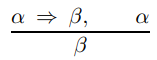
\includegraphics[]{images/modus-ponens.png}
\end{center}
The notation means that, whenever any sentences of the form $\alpha \Rightarrow \beta$ and $\alpha$ are given, then the sentence $\beta$ can be inferred. For example, if $(WumpusAhead \land WumpusAlive) \Rightarrow Shoot$ and $(WumpusAhead \land WumpusAlive)$ are given, then $Shoot$ can be inferred. These techniques typically require translation of sentences into a \textbf{normal form}.
\newline\newline
Some real-world knowledge bases satisfy certain restrictions on the form of sentences they contain, which enables them to be represented with a restricted form which enables more efficient inference algorithms. One such restricted form is the \textbf{Horn form}, which is a conjunction of Horn clauses. A Horn clause is defined as follows:
\begin{itemize}
    \item proposition symbol; or
    \item (conjunction of symbols) $\Rightarrow$ symbol.
    \[C \land (B \Rightarrow A) \land (C \land B \Rightarrow A)\]
\end{itemize}
In Horn form, the premise is called the \textbf{body} and the conclusion is called the \textbf{head}. A sentence consisting of a single positive literal, such as $P_{1,1}$, is called a \textbf{fact} ($True \Rightarrow P_{1,1}$).\newline\newline
Knowledge bases containing only Horn clauses are interesting for the following reasons:
\begin{itemize}
    \item  Inference with Horn clauses can be done through the forward-chaining and backwardchaining algorithms, which we explain next. Both of these algorithms are natural, in that the inference steps are obvious and easy for humans to follow.

    \item  Deciding entailment with Horn clauses can be done in time that is linear in the size of the knowledge base.
\end{itemize}

\section{Forward and Backward Chaining}
The \textbf{forward-chaining} algorithm  determines if a single proposition symbol $q$, the query, is entailed by a knowledge base of Horn clauses. It begins from known facts in the knowledge base. If all the premises of an implication are known, then its conclusion is added to the set of known facts. For example, if $L_{1,1}$ and $Breeze$ are known and $(L_{1,1} \land Breeze) \Rightarrow B_{1,1}$ is in the knowledge base, then $B_{1,1}$ can be added. This process continues until the query $q$ is added or until no further inferences can be made.
\begin{center}
    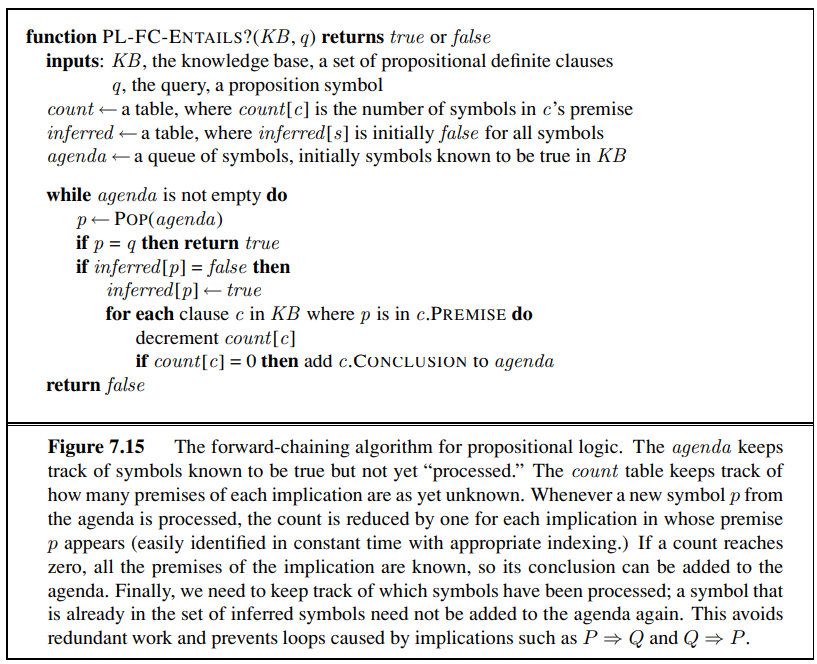
\includegraphics[]{images/forward chaining.png}
    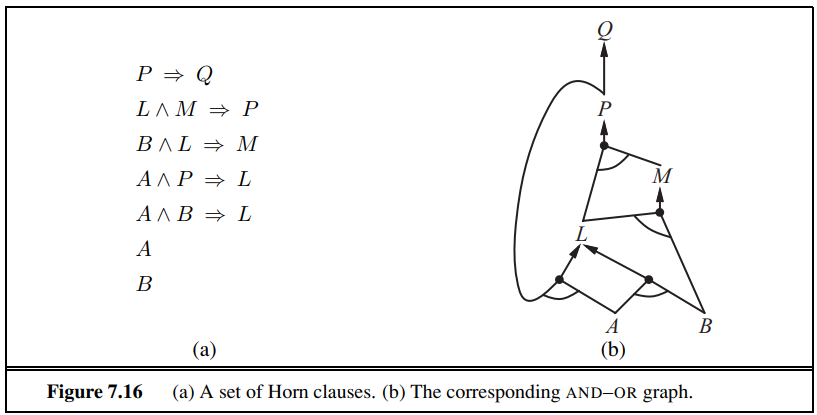
\includegraphics[]{images/graph.png}
\end{center}
The best way to understand the algorithm is through an example showed in the figure above. It shows a simple knowledge base of Horn clauses with $A$ and $B$ as known facts represented as an AND-OR graph. In AND–OR graphs, multiple links joined by an arc indicate a conjunction, that is, every link must be proved. While multiple links without an arc indicate a disjunction, any link can be proved.
\begin{center}
    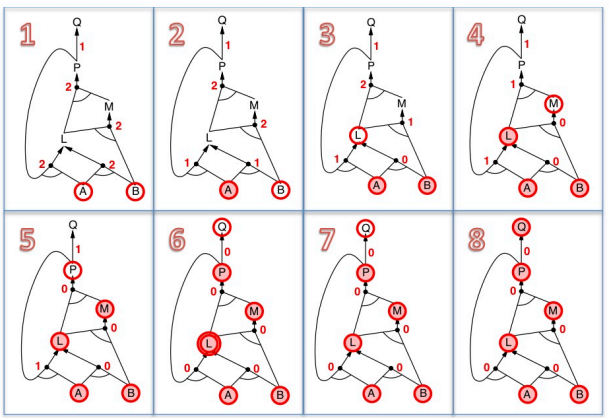
\includegraphics[]{images/frwd exec.png}
\end{center}
Forward chaining is \textbf{sound}: every inference is essentially an application of Modus Ponens. Forward chaining is also \textbf{complete}: every entailed atomic sentence will be derived.\newline\newline
The easiest way to see this is to consider the final state of the \textit{inferred} table (after the algorithm reaches a \textbf{fixed point} where no new inferences are possible). The table contains \textit{true} for each symbol inferred during the process, and \textit{false} for all other symbols. We can view the table as a logical model; moreover, every Horn clause in the original KB is true in this model. To see this, assume the opposite, namely that some clause $a_1\land ...\land a_k \Rightarrow b$ is \textit{false} in the model. Then $a_1\land ...\land a_k$ must be \textit{true} in the model and $b$ must be \textit{false} in the model. But this contradicts our assumption that the algorithm has reached a fixed point. We can conclude, therefore, that the set of atomic sentences inferred at the fixed point defines model of the original KB. Furthermore, any atomic sentence $q$ that is entailed by the KB must be true in all its models and in this model in particular. Hence, every entailed atomic sentence $q$ must be inferred by the algorithm.\newline\newline
The \textbf{backward-chaining} algorithm, as its name suggests, works backward from the query.  If the query $q$ is known to be true, then no work is needed. Otherwise, the algorithm finds those implications in the knowledge base whose conclusion is $q$.  If all the premises of
one of those implications can be proved true (by backward chaining), then $q$ is true.
\begin{center}
    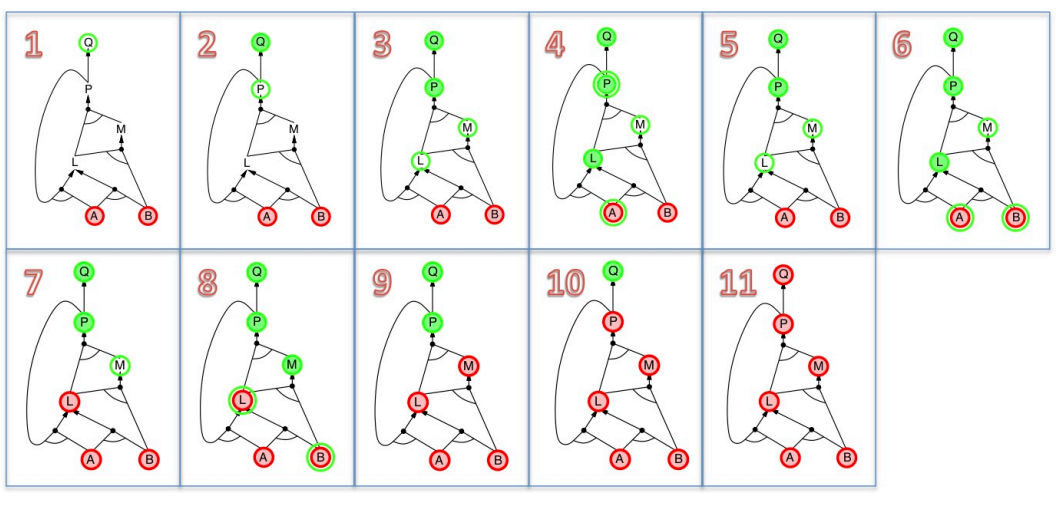
\includegraphics[scale=0.8]{images/bkwrd exec.png}
\end{center}
Forward chaining is an example of the general concept of \textbf{data-driven} reasoning, that is, reasoning in which the focus of attention starts with the known data. However, it may do lots of work that is irrelevant to the goal.\newline\newline
Backward chaining is a form of \textbf{goal-directed} reasoning. It is appropriate for problem solving and for answering specific questions such as “What shall I do now?” and “Where are my keys?" Often, the cost of backward chaining is much less than linear in the size of the knowledge base, because the process touches only relevant facts.

\section{Resolution}
The current section introduces a single inference rule, \textbf{resolution}, that yields a complete inference algorithm when coupled with any complete search algorithm. The resolution rule applies only to disjunctions of literals (clauses), so it would seem
to be relevant only to knowledge bases and queries consisting of clauses. How, then, can it lead to a complete inference procedure for all of propositional logic?  The answer is that every sentence of propositional logic is logically equivalent to a \textbf{conjunction of clauses}. A sentence expressed as a conjunction of clauses is said to be in \textbf{conjunctive normal form} or \textbf{CNF}.\newline\newline
The resolution rule is the following:
\begin{center}
    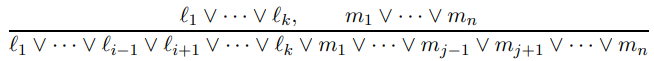
\includegraphics[]{images/resolution.png}
\end{center}
where $l_i$ and $m_j$ are complementary literals. This says that resolution takes two clauses and produces a new clause containing all the literals of the two original clauses except the two complementary literals. For example:
\begin{center}
    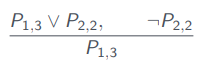
\includegraphics[]{images/resolution-wumpus.png}
\end{center}
means that if there is a pit in $[1,3]$ or in $[2,2]$ and the pit is not in $[2,2]$, then the pit is in $[1,3]$.\newline\newline
The soundness of the resolution rule can be seen easily by considering the literal $l_i$ that is complementary to literal $m_j$ in the other clause. If $l_i$ is true, then $m_j$ is false, and hence $m_1 \lor ... \lor m_{j-1} \lor m_{j+1} \lor ... \lor m_n$ must be true, because $m_1 \lor ... \lor m_n$ is \textbf{given}. If $l_i$ is false, then $l_1 \lor ... \lor l_{i-1} \lor l_{i+1} \lor ... \lor l_k$ must be true, because $l_1 \lor ... \lor l_k$ is given. Therefore, every derived sentence is also entailed.\newline\newline
What is more surprising about the resolution rule is that it forms the basis for a family
of complete inference procedures. A resolution-based theorem prover can, for any sentences
$\alpha$ and $\beta$ in propositional logic, decide whether $\alpha \vDash \beta$.

\subsection{A resolution algorithm}
Inference procedures based on resolution work by using the principle of proof by contradiction, that is, to show that $KB \vDash \alpha$, we show that $KB \land \neg{\alpha}$ is unsatisfiable.
\begin{center}
    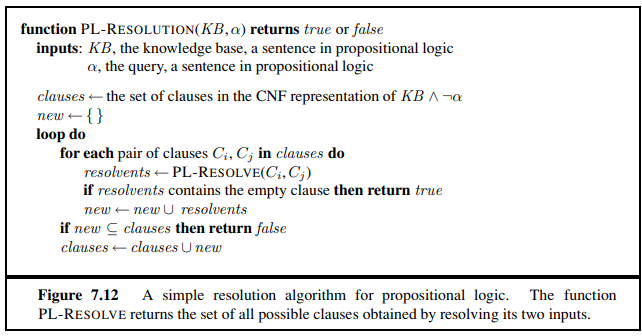
\includegraphics[]{images/resolution algorithm.png}
\end{center}
First, $(KB \land \neg{\alpha})$ is converted into CNF. Then, the resolution rule is applied to the resulting clauses. Each pair that contains complementary literals is resolved to produce a new clause, which is added to the set if it is not already present. The process continues until one of two things happens:
\begin{itemize}
    \item there are no new clauses that can be added, in which case KB does not entail $\alpha$; or,

    \item two clauses resolve to yield the empty clause, in which case KB entails $\alpha$. 
\end{itemize}
Note that the empty clause, a disjunction of no disjuncts, is equivalent to \textit{False}, because a disjunction is true only if at least one of its disjuncts is true.
\begin{center}
    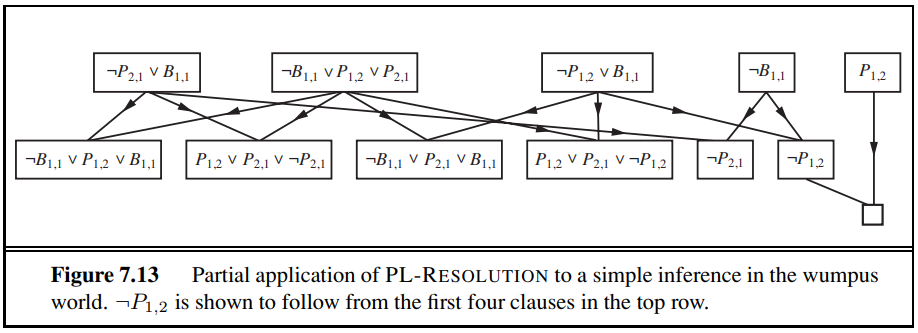
\includegraphics[]{images/resolution-wumpus2.png}
\end{center}
We can apply the resolution procedure to a very simple inference in the wumpus world. When the agent is in $[1,1]$, there is no breeze, so there can be no pits in neighboring squares. The relevant knowledge base is:
\begin{center}
    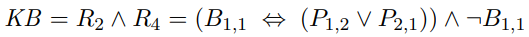
\includegraphics[]{images/wumpus-kb.png}
\end{center}
When we convert $(KB \land \neg{\alpha})$ into CNF, we obtain the clauses shown at the top of the figure above. The second row of the figure shows clauses obtained by resolving pairs in the first row. Then, when $P_{1,2}$ is resolved with $\neg{P_{1,2}}$, we obtain the empty clause, shown as a small square. Therefore, we can deduce that $KB \vDash \neg{P_{1,2}}$.

\subsection{Completeness of Resolution Algorithm}
To conclude our discussion of resolution, we now show why PL-RESOLUTION is complete. To do this, we introduce the \textbf{resolution closure} $RC(S)$ of a set of clauses $S$, which is the set of all clauses derivable by repeated application of the resolution rule to clauses in $S$ or their
derivatives. The resolution closure is what PL-RESOLUTION computes as the final value of the variable \textit{clauses}.\newline\newline
The completeness theorem for resolution in propositional logic is called the \textbf{ground resolution theorem}: \textit{If a set of clauses is unsatisfiable, then the resolution closure of those clauses contains the empty clause}.
\newline\newline
This theorem is proved by demonstrating its contrapositive: if the closure $RC(S)$ does \textbf{not} contain the empty clause, then $S$ is satisfiable. In fact, we can construct a model for $S$ with suitable truth values for $P_1, ..., P_k$. The construction procedure is as follows:\newline\newline
For $i$ from 1 to $k$,
\begin{itemize}
    \item If a clause in $RC(S)$ contains the literal $\neg{P_i}$ and all its other literals are false under the assignment chosen for $P_1, ... P_{i-1}$, then assign false to $P_i$.

    \item Otherwise, assign true to $P_i$.
\end{itemize}
This assignment to $P_1,...,P_k$ is a model of $S$. To see this, assume the opposite, that, at some stage $i$ in the sequence, assigning symbol $P_i$ causes some clause $C$ to become false. For this to happen, it must be the case that all the other literals in $C$ must already have been falsified by assignments to $P_1,...,P_{i-1}$. Thus, $C$ must now look like either $(false \lor false \lor ... false \lor P_i)$ or like $(false \lor false \lor ... false \lor \neg{P_i})$.  If just one of these two is in $RC(S)$, then the procedure will assign the appropriate truth value to $P_i$ to make $C$ true, so $C$ can only be falsified if both of these clauses are in $RC(S)$.  Now, since $RC(S)$ is closed under resolution, it will contain the resolvent of these two clauses, and that resolvent will have all of its literals already falsified by the assignments to $P_1,...,P_{i-1}$. This contradicts our assumption that the first falsified clause appears at stage $i$. Hence, we have proved that the construction never falsifies a clause in $RC(S)$,  that is, it produces a model of $RC(S)$. 
